\subsubsection*{8.}
Pour vérifier s'il y a une référence de la table \texttt{SUBSCRIBE} dans la table \texttt{THING},
nous allons effectuer une jointure de la table \texttt{USER\_CONSTRAINTS} avec elle-même. Nous 
utilisons un \textit{select imbriqué} ou la \textit{sous-requête} récupère les noms
des contraintes référencées de la table \texttt{THING}, c'est-à-dire les contraintes de clé
primaire des table references par \texttt{THING}. La requête principale compte ensuite le nombre de contraintes de 
clé primaire dans la table \texttt{SUBSCRIBE} qui figurent parmi les contraintes obtenues dans la sous-requête. 
si count = 0 , pas de references sinon si 1 ya une reference 

\lstinputlisting[style=sqlstyle]{SQL/Partie5/fr.sql}

\begin{center}
    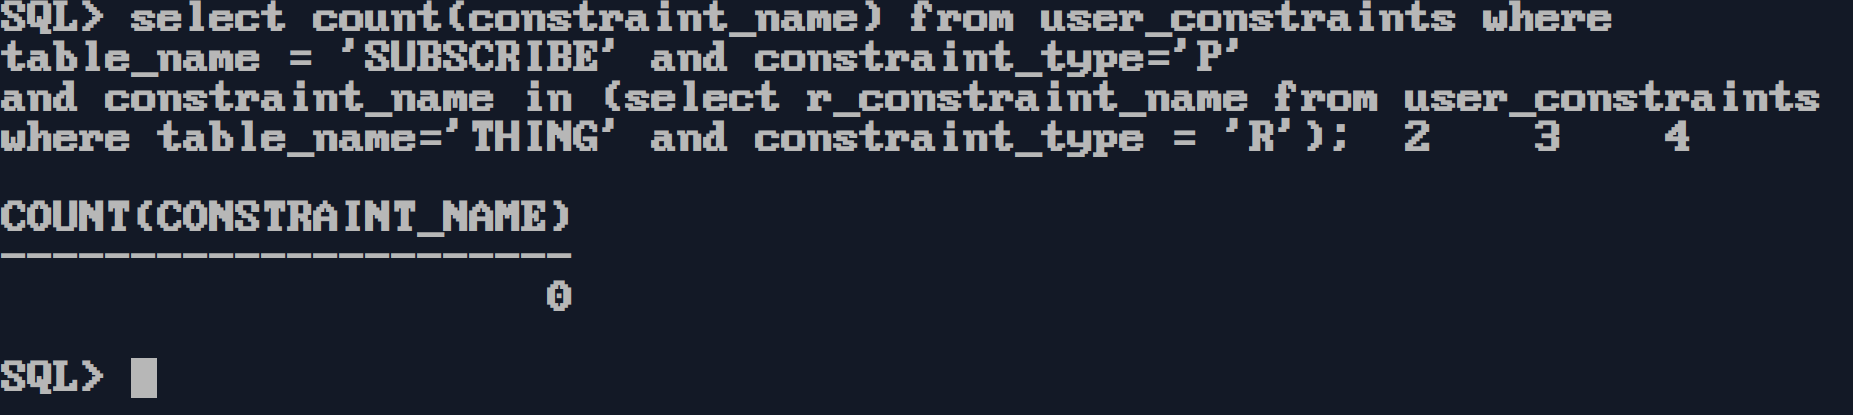
\includegraphics[width=\textwidth]{ScreenShot/Partie5/fr.png}
\end{center}

\begin{prettyBox}{Remarque}{myblue}
\begin{itemize}
    \item Constraint\_Type = 'R' : contrainte cle etrangere
    \item Constraint\_Type = 'P' : contrainte cle primaire
    \item R\_Constraint\_Name : nom des contrainte cle primaire reference par la table
\end{itemize}
\end{prettyBox}


